\documentclass[a4paper, 12pt]{article}
\usepackage{tikz}
\usetikzlibrary{positioning, arrows.meta, fit, backgrounds, calc}
\usepackage{xcolor}
\usepackage{float}
\usepackage{caption}
\usepackage{geometry}
\geometry{margin=1.5cm, landscape}

\begin{document}
\pagestyle{empty}

\begin{figure}[H]
\centering
{\large\bfseries\sffamily Figure 3: System Architecture Diagram}\\[4pt]
{\normalsize\sffamily Re-scaled with smaller fonts and boxes to eliminate congestion and tight spacing.}
\vspace{10pt}

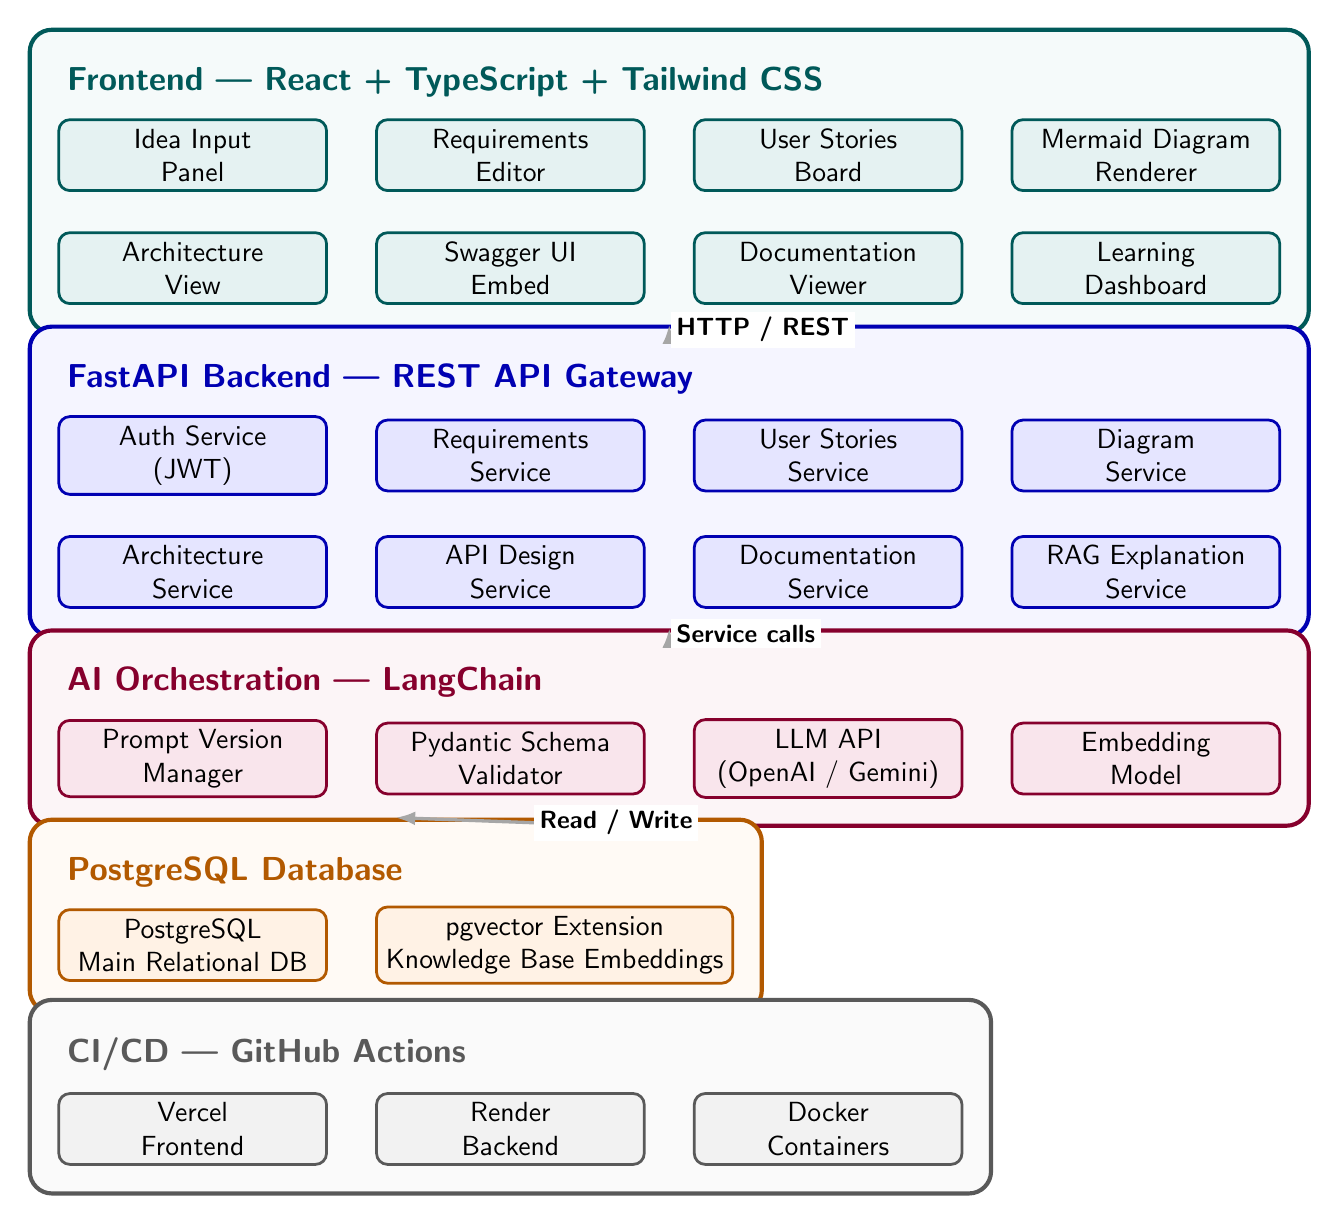
\begin{tikzpicture}[
  node distance=0.5cm and 0.6cm,
  box/.style={rectangle, draw=#1!70!black, fill=#1!10,
              rounded corners=4pt, minimum width=3.4cm,
              minimum height=0.8cm, align=center,
              font=\normalsize\sffamily, line width=1pt},
  layer/.style={rectangle, draw=#1!70!black, fill=#1!4,
                rounded corners=8pt, line width=1.5pt,
                inner sep=10pt},
  layerlabel/.style={font=\large\bfseries\sffamily, text=#1!70!black},
  arrow/.style={-{Latex[length=7pt, width=5pt]}, line width=1.2pt, draw=gray!70},
  arrlbl/.style={font=\small\bfseries\sffamily, fill=white, inner sep=2pt}
]

% ==================== FRONTEND LAYER ====================
\node[box=teal] (ui1) {Idea Input\\Panel};
\node[box=teal, right=of ui1] (ui2) {Requirements\\Editor};
\node[box=teal, right=of ui2] (ui3) {User Stories\\Board};
\node[box=teal, right=of ui3] (ui4) {Mermaid Diagram\\Renderer};
\node[box=teal, below=of ui1] (ui5) {Architecture\\View};
\node[box=teal, right=of ui5] (ui6) {Swagger UI\\Embed};
\node[box=teal, right=of ui6] (ui7) {Documentation\\Viewer};
\node[box=teal, right=of ui7] (ui8) {Learning\\Dashboard};

\node[layerlabel=teal, above left=0.15cm and 0cm of ui1.north west, anchor=south west] (felabel) 
  {Frontend --- React + TypeScript + Tailwind CSS};

\begin{pgfonlayer}{background}
  \node[layer=teal, fit=(felabel)(ui1)(ui4)(ui5)(ui8)] (felayer) {};
\end{pgfonlayer}

% ==================== BACKEND LAYER ====================
\node[box=blue, below=1.4cm of ui5] (b1) {Auth Service\\(JWT)};
\node[box=blue, right=of b1]     (b2) {Requirements\\Service};
\node[box=blue, right=of b2]     (b3) {User Stories\\Service};
\node[box=blue, right=of b3]     (b4) {Diagram\\Service};
\node[box=blue, below=of b1] (b5) {Architecture\\Service};
\node[box=blue, right=of b5]     (b6) {API Design\\Service};
\node[box=blue, right=of b6]     (b7) {Documentation\\Service};
\node[box=blue, right=of b7]     (b8) {RAG Explanation\\Service};

\node[layerlabel=blue, above left=0.15cm and 0cm of b1.north west, anchor=south west] (belabel) 
  {FastAPI Backend --- REST API Gateway};

\begin{pgfonlayer}{background}
  \node[layer=blue, fit=(belabel)(b1)(b4)(b5)(b8)] (belayer) {};
\end{pgfonlayer}

% ==================== AI LAYER ====================
\node[box=purple, below=1.4cm of b5] (ai1) {Prompt Version\\Manager};
\node[box=purple, right=of ai1] (ai2) {Pydantic Schema\\Validator};
\node[box=purple, right=of ai2] (ai3) {LLM API\\(OpenAI / Gemini)};
\node[box=purple, right=of ai3] (ai4) {Embedding\\Model};

\node[layerlabel=purple, above left=0.15cm and 0cm of ai1.north west, anchor=south west] (ailabel) 
  {AI Orchestration --- LangChain};

\begin{pgfonlayer}{background}
  \node[layer=purple, fit=(ailabel)(ai1)(ai4)] (ailayer) {};
\end{pgfonlayer}

% ==================== DATABASE LAYER ====================
\node[box=orange, below=1.4cm of ai1] (db1) {PostgreSQL\\Main Relational DB};
\node[box=orange, right=of db1] (db2) {pgvector Extension\\Knowledge Base Embeddings};

\node[layerlabel=orange, above left=0.15cm and 0cm of db1.north west, anchor=south west] (dblabel) 
  {PostgreSQL Database};

\begin{pgfonlayer}{background}
  \node[layer=orange, fit=(dblabel)(db1)(db2)] (dblayer) {};
\end{pgfonlayer}

% ==================== CI/CD LAYER ====================
\node[box=gray, below=1.4cm of db1] (ci1) {Vercel\\Frontend};
\node[box=gray, right=of ci1] (ci2) {Render\\Backend};
\node[box=gray, right=of ci2] (ci3) {Docker\\Containers};

\node[layerlabel=gray, above left=0.15cm and 0cm of ci1.north west, anchor=south west] (cilabel) 
  {CI/CD --- GitHub Actions};

\begin{pgfonlayer}{background}
  \node[layer=gray, fit=(cilabel)(ci1)(ci3)] (cilayer) {};
\end{pgfonlayer}

% ==================== ARROWS ====================
\draw[arrow] (felayer.south) -- node[arrlbl, right]{HTTP / REST} (belayer.north);

\draw[arrow] (belayer.south) -- node[arrlbl, right]{Service calls} (ailayer.north);

\draw[arrow] (ailayer.south) -- node[arrlbl, right]{Read / Write} (dblayer.north);

\end{tikzpicture}
\end{figure}

\end{document}
